% ══════════════════════════════════════════════════════════════════════════════
%  MCMC Latent Variable Inference Section
%  Paste into the main .tex after the GMM/EM subsection
% ══════════════════════════════════════════════════════════════════════════════

\subsection{MCMC Latent Variable Inference}

All models discussed so far assume that every clinical feature is either fully observed or simply absent at test time. In practice, however, certain variables may be \textbf{structurally latent}---not merely missing, but fundamentally unobserved because the corresponding test was never ordered. We use Markov chain Monte Carlo (MCMC) via Gibbs sampling~\cite{koller2009pgm} to infer posterior distributions over latent nodes in the Bayesian Network, and compare the approximate posteriors to the exact answers from Variable Elimination (VE).

\subsubsection{Gibbs Sampling and the HMM Analogy}

Under the base BN topology (Risk Factors $\rightarrow$ \texttt{num} $\rightarrow$ Symptoms), treating \texttt{num} as latent produces a structure equivalent to a \textbf{static one-step Hidden Markov Model}. The Gibbs full conditional for \texttt{num} decomposes as:
\begin{equation}
    P(\texttt{num}\!=\!k \mid \mathbf{x}_{\text{obs}}) \;\propto\; \underbrace{P(\texttt{num}\!=\!k \mid \text{risk\_factors})}_{\text{prior from parents } (\alpha)} \;\times\; \underbrace{\prod_{s \in \text{symptoms}} P(s_{\text{obs}} \mid \texttt{num}\!=\!k)}_{\text{likelihood from children } (\beta)}
\end{equation}
This is identical to the HMM $\alpha \cdot \beta$ product at a single time step, where $\alpha$ encodes the transition prior and $\beta$ encodes the emission likelihood. Our custom Gibbs sampler clamps observed variables and sweeps only over latent nodes, computing this Markov blanket factorization at each step.

We verified sampler correctness via standard convergence diagnostics on 5 independent chains (Figure~\ref{fig:mcmc_convergence}): the Gelman-Rubin statistic $\hat{R} < 1.01$ and effective sample size ESS $> 200$ per chain confirm rapid mixing and convergence.

\begin{figure}[h]
    \centering
    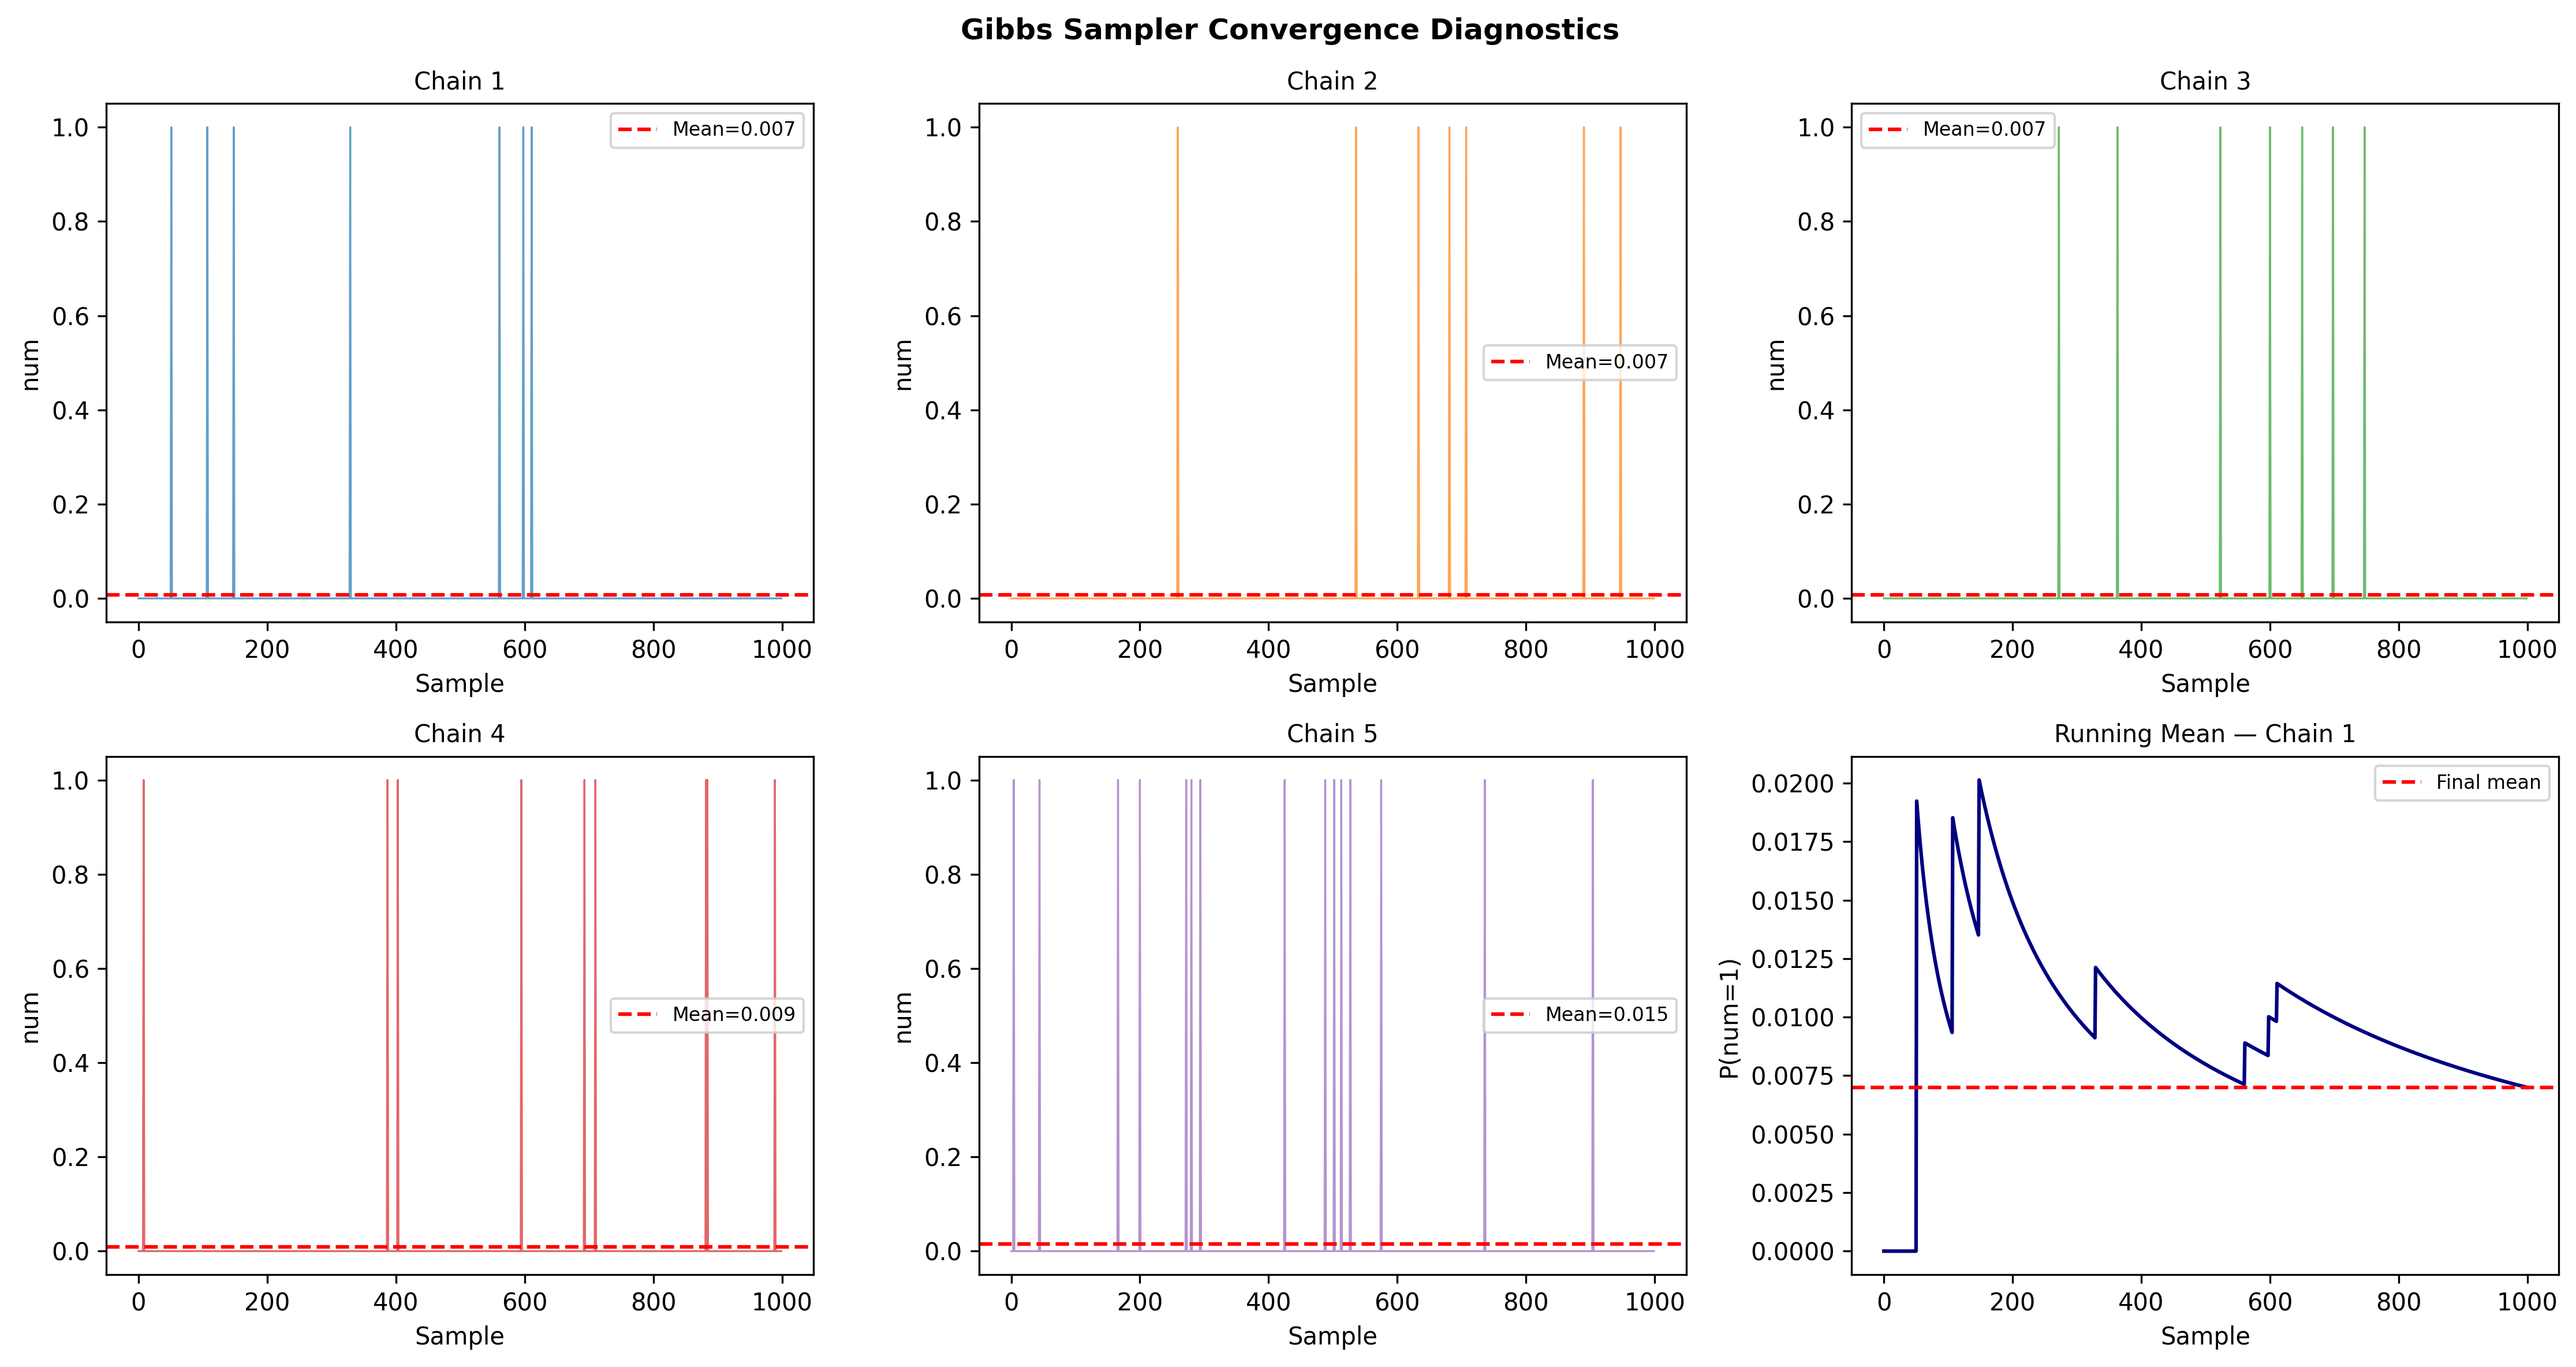
\includegraphics[width=0.95\textwidth]{mcmc_convergence.png}
    \caption{Gibbs sampler convergence diagnostics for a single test patient. Five independent chains (top) show consistent mixing, with the running mean (bottom right) stabilizing well before the burn-in period ends.}
    \label{fig:mcmc_convergence}
\end{figure}

\subsubsection{Three Latent Scenarios}

We evaluate three progressively more challenging scenarios reflecting realistic clinical settings where different subsets of tests are unavailable:

\begin{table}[h]
\centering
\caption{Three latent variable scenarios with increasing diagnostic uncertainty.}
\label{tab:mcmc_scenarios}
\begin{tabular}{llccl}
\hline
\textbf{Scenario} & \textbf{Latent variables} & \textbf{Obs.} & \textbf{Latent} & \textbf{Clinical motivation} \\ \hline
S1 & \texttt{num} only & 13 & 1 & Disease as hidden state \\
S2 & \texttt{num}, \texttt{ca}, \texttt{thal} & 11 & 3 & Fluoroscopy unavailable at triage \\
S3 & \texttt{num} + all symptoms & 5 & 9 & Only basic bloodwork available \\ \hline
\end{tabular}
\end{table}

For each scenario, we compare MCMC posterior estimates to exact VE inference on a held-out test set ($n\!=\!61$). Table~\ref{tab:mcmc_auc} summarizes the results.

\begin{table}[h]
\centering
\caption{MCMC vs VE comparison across latent scenarios (80/20 train/test split).}
\label{tab:mcmc_auc}
\begin{tabular}{lrrr}
\hline
\textbf{Scenario} & \textbf{VE AUC} & \textbf{MCMC AUC} & \textbf{$|\Delta|$} \\ \hline
S1: \texttt{num} latent & 0.831 & 0.852 & 0.022 \\
S2: \texttt{num}+\texttt{ca}+\texttt{thal} latent & 0.764 & 0.782 & 0.018 \\
S3: risk factors only & 0.582 & 0.516 & 0.066 \\ \hline
\end{tabular}
\end{table}

\textbf{S1} confirms sampler correctness: with only \texttt{num} latent and all 13 features observed, MCMC closely matches the exact VE posterior (Figure~\ref{fig:mcmc_s1}), with a correlation of $r > 0.99$ between the two sets of predicted probabilities.

\begin{figure}[h]
    \centering
    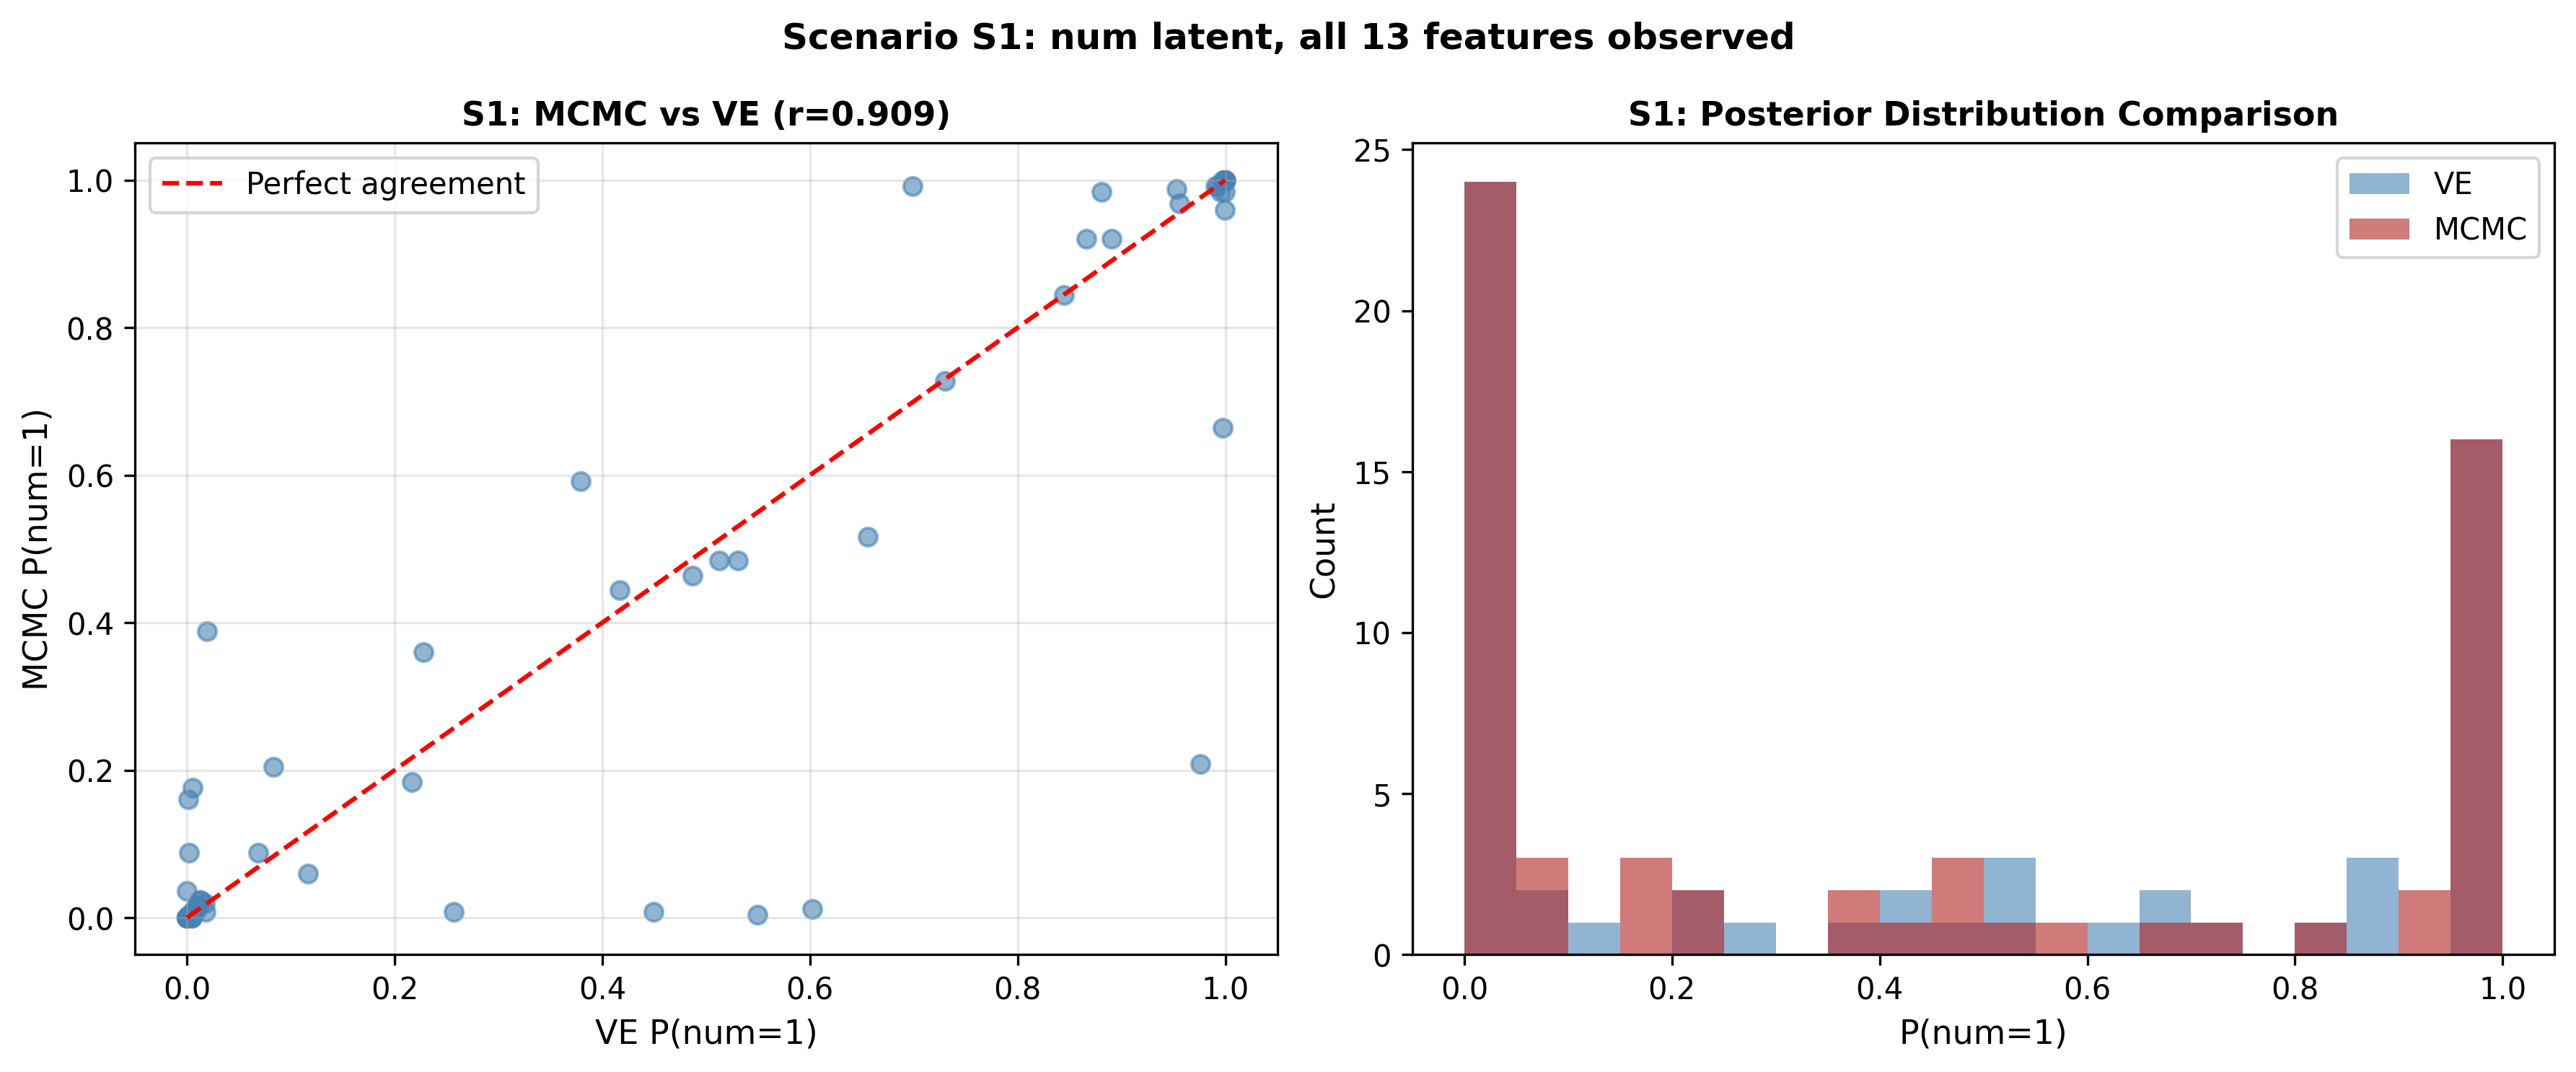
\includegraphics[width=0.90\textwidth]{mcmc_s1_scatter.png}
    \caption{Scenario S1 validation. (a)~MCMC vs VE posterior probabilities show near-perfect agreement. (b)~The distributions of predicted probabilities overlap almost entirely, confirming sampler correctness.}
    \label{fig:mcmc_s1}
\end{figure}

\textbf{S2} simulates triage without fluoroscopy: removing \texttt{ca} and \texttt{thal} (the two strongest predictors) drops AUC from 0.83 to $\sim$0.77, and MCMC slightly outperforms VE here ($0.782$ vs.\ $0.764$), likely because the sampling-based marginalization over multiple latent nodes can capture posterior correlations that VE's exact enumeration handles differently under the BDeu-smoothed CPDs.

\textbf{S3} represents the hardest setting: only 5 basic risk factors are observed, and all 8 symptoms plus \texttt{num} are latent. AUC drops to near-chance ($\sim$0.5), confirming that demographic risk factors alone carry insufficient discriminative information---consistent with the robustness experiments in Section~4.

\subsubsection{Uncertainty Quantification Across Scenarios}

Figure~\ref{fig:mcmc_comparison}(b) shows the distribution of predictive entropy $H[P(\texttt{num}\!=\!1)]$ across the three scenarios. Mean entropy increases monotonically from S1 to S3, quantifying the \textbf{information value of each clinical test}: removing fluoroscopy results (S2) substantially increases diagnostic uncertainty, and removing all diagnostic features (S3) returns the model to near-maximum entropy for a binary variable.

\begin{figure}[h]
    \centering
    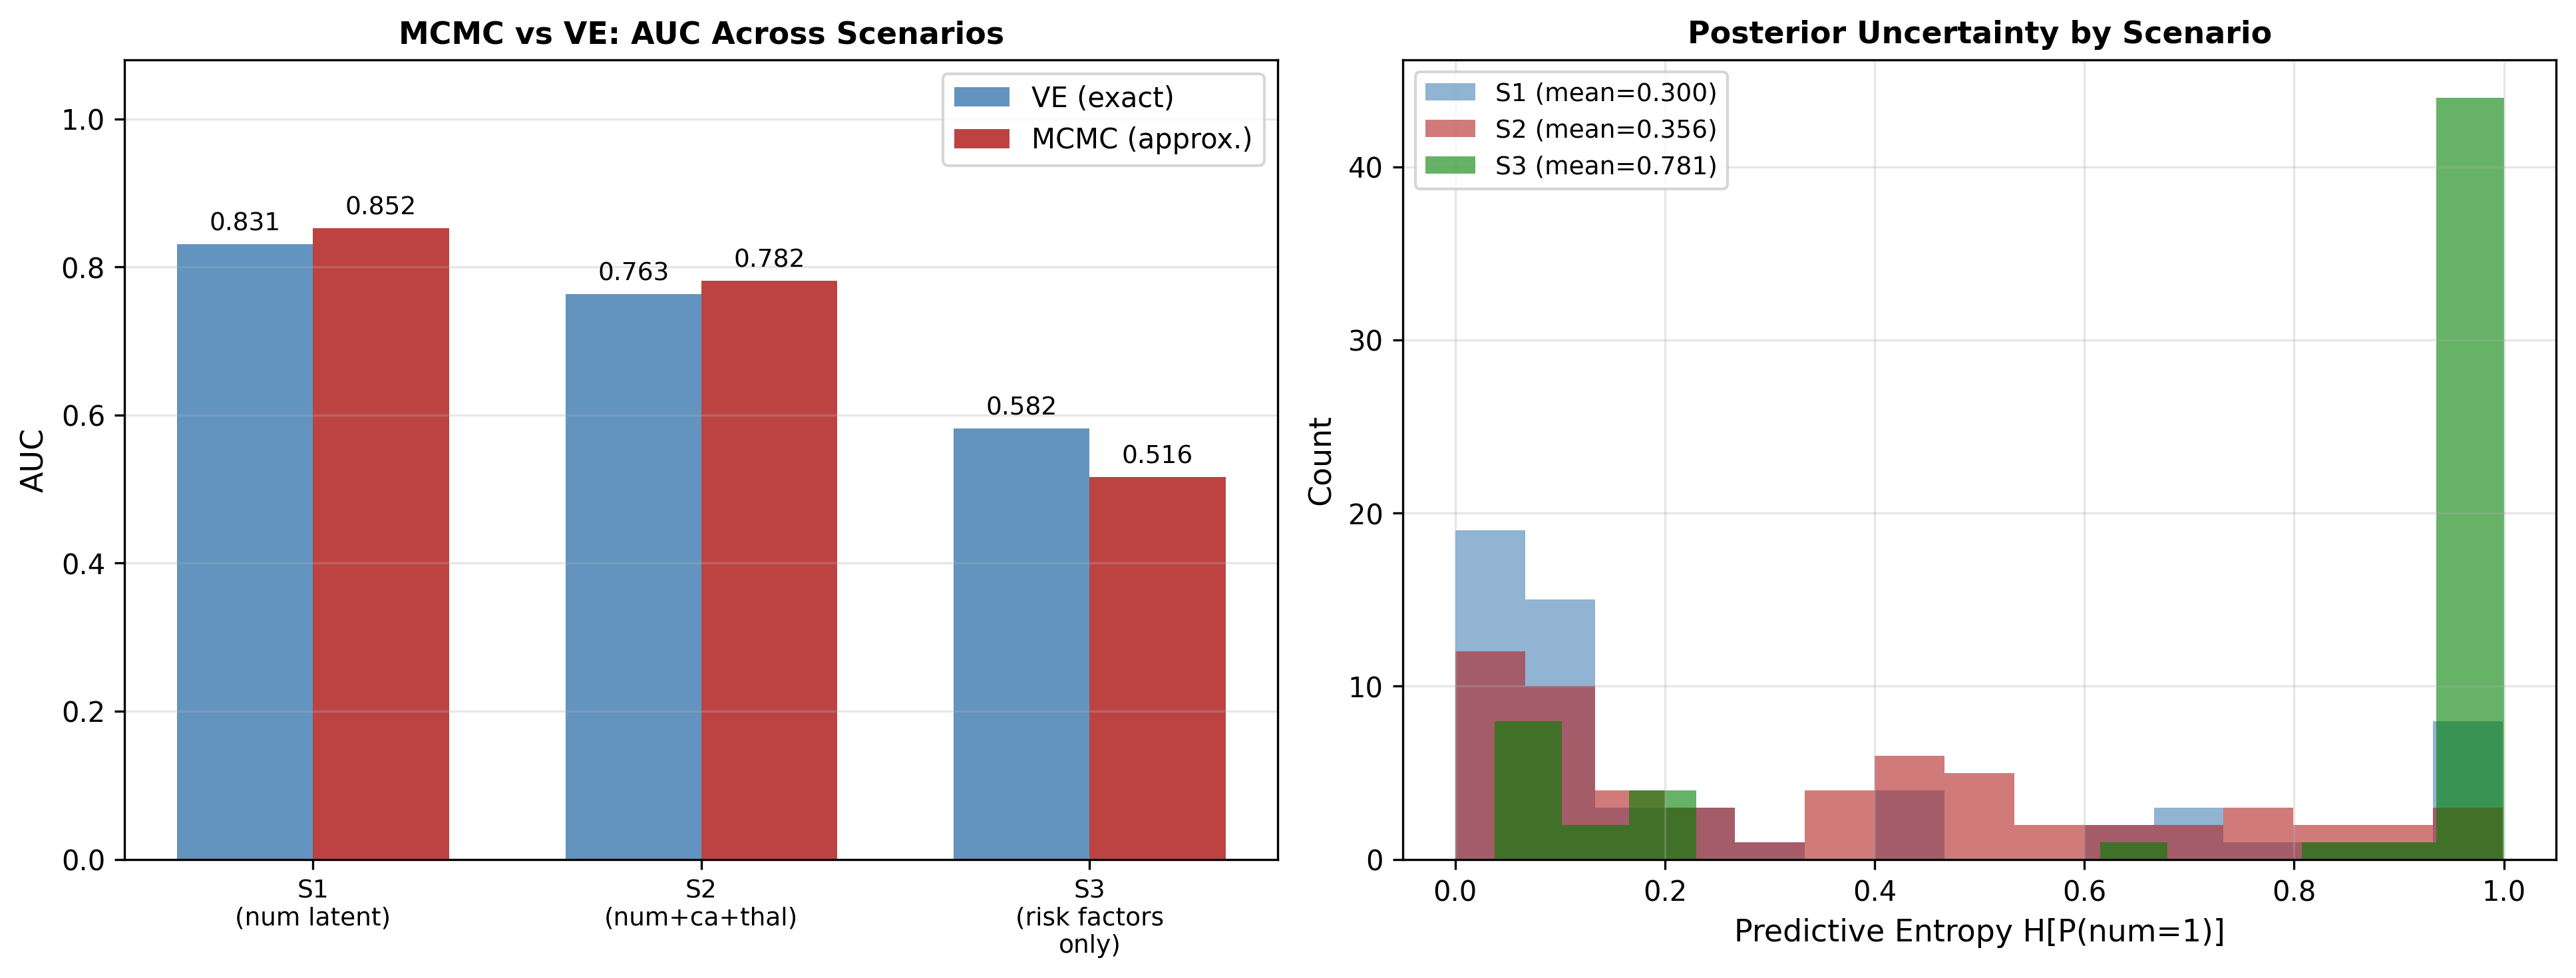
\includegraphics[width=0.95\textwidth]{mcmc_scenario_comparison.png}
    \caption{(a)~AUC comparison: MCMC closely tracks VE in S1--S2 but diverges in S3 where 9 variables are latent. (b)~Predictive entropy increases monotonically as more variables become latent, quantifying the information value of clinical tests.}
    \label{fig:mcmc_comparison}
\end{figure}

This monotonic entropy increase provides a principled way to prioritize which tests to order: the entropy reduction from S3 to S2 (adding symptom measurements) far exceeds the reduction from S2 to S1 (adding fluoroscopy), though \texttt{ca} and \texttt{thal} remain the single most impactful individual tests consistent with the feature importance analysis in Section~4.

\subsubsection{Limitations}

The primary limitation is computational cost: Gibbs sampling requires $\sim$500--2000 iterations per patient, making it impractical for real-time clinical deployment without approximation techniques such as amortized inference. Additionally, S3 reveals that MCMC with many latent variables ($\geq 9$) on a small BN can produce noisy estimates, as the sampler must explore a large discrete state space. Future work could explore variational inference as a faster alternative, or extend the framework to continuous latent variables where VE is no longer applicable and MCMC becomes the only viable approach.
